% Chapter 1

\chapter{Introduction} % Main chapter title

\label{Chapter1} % For referencing the chapter elsewhere, use \ref{Chapter1} 

\lhead{Chapter 1. \emph{Introduction}} % This is for the header on each page - perhaps a shortened title

\section{Purpose/Motivation}
It is no secret that elderly population is in a constant rise, currently 15\% of the norwegian population is above the age of 65. By the turn of the century the elderly population is expected to double \cite{elder}. The initial rise of the elder population will be most noticable in those below the age of 80, as seen in figure \ref{fig:elderPopulation}. Whereas we will see a great spike in the above 80 population after 2025. The publication reports that two out of three above the age of 75 consider themselves having "good health" but only a third preserve this level of health until death.

\begin{figure}[h!]
	\centering
		\label{fig:elderPopulation}
		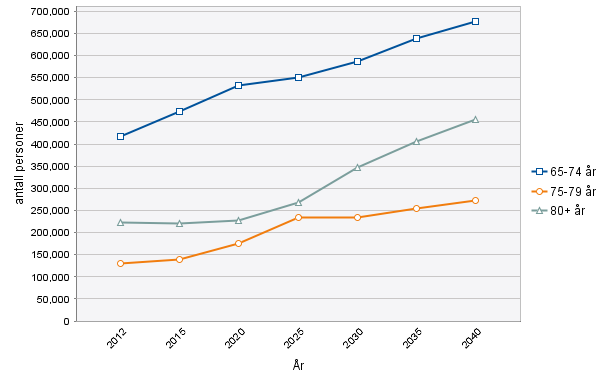
\includegraphics[width=0.5\textwidth]{eldrevekst.png}
		\caption{\footnotesize Elder population estimation \cite{elder}}
\end{figure}

One of the largest ever systematic efforts to describe the global health situation was conducted in 2010. One of their many findings was that since 1970 men and women have gained an additional ten years to their life expectancy, but spend more time living with injuries and illness \cite{globalBurden}. %KOMMER TILBAKE HIT

In the late 1990s the Norwegian statistical bureau published a paper predicting a major increase in the elderly population, the working population compared to the retired currently holds a ratio of 5 to 1. This is expected to drop below 3 by the year 2040. Due to this the greatest challenges within wellfare are expected to occur between 1998 and 2020 \cite{eldreEksplosjon}. 

With such predictions the Norwegian government formed a committee (often refered to as Hagenutvalget*) that would investigate the current situation and look at possible solutions \cite{haagen}. The most relevant conclusion was that too little of today's technology is incorporated as welfare technology* for the elderly. A Danish report states that around 20\% of the tasks could be completely or partly replaced by technology \cite{kmd}. If the Norwegian circumstances are similar this could lead to great savings in the health budget.

Hagenutvalget suggest a national three step program that focus on using welfare technology to diminish falls, social isolation and cognitive failure. Thus improving the overall quality of life for the elder population. The step of most relevance to our work is step 3:

\epigraph{\textit{``Step 3: Opt on technology that stimulates, activates and structures daily life.''}}{--- \textup{NOU 2011: 11}}


\section{Project context/Thesis Scope}
This project is a cooperation between the Department of Computer and Information Science (IDI)* at the Norwegian University of Science and Technology(NTNU) and St. Olavs University Hospital in Trondheim. The project....

\section{Research questions}

\section{Research method}

\section{Thesis outline}